\documentclass{article}
%%%%%%%%%%%%
% PACKAGES %
%%%%%%%%%%%%
\usepackage[utf8]{inputenc}
\usepackage{lastpage}

\usepackage{todonotes}

\usepackage[urldate=long]{biblatex}
\addbibresource{references.bib}
\usepackage[hidelinks]{hyperref}

% Changes the paragraph indentations to newlines
\usepackage[parfill]{parskip}

\usepackage[a4paper]{geometry}

\usepackage{minted}
% \usemintedstyle{vs}
\newenvironment{haskell}{\VerbatimEnvironment\begin{center}\begin{minted}[escapeinside=!!]{haskell}}{\end{minted}\end{center}}

\newcommand{\inlinehaskell}[1]{\mintinline[escapeinside=!!]{haskell}{#1}}

\usepackage{float}

\usepackage{graphicx}
\graphicspath{ {images} }

\usepackage{fancyhdr}
\pagestyle{fancy}
\fancyhf{} % Clears the default header and footers
\fancyhead[L]{Jort van Gorkum — Master's Thesis}
\fancyhead[R]{Page \thepage\ of \pageref{LastPage}}

\linespread{1.2}

\usepackage[inline]{enumitem}

\usepackage{multirow}

%%%%%%%%%%%%
% DOCUMENT %
%%%%%%%%%%%%
\begin{document}

\begin{titlepage}
    \fontsize{12pt}{15pt}\selectfont
    \begin{center}
      \vspace*{4cm}
  
      Master's Thesis
  
      \vspace{0.5cm}
  
      {
        \fontsize{20.74pt}{20.74pt}\selectfont
        \parbox[]{13cm} {
          \centering
          Incremental Cata Computation \\ for Generic Data Types
        }
      }
        
      \vspace{1.25cm}
      
      Jort van Gorkum - 6142834 \\
      Computing Science - Programming Technology \\
      Utrecht University \\
      
      \vspace{1.25cm}
      
      Supervisors: \\
      Dr. Wouter Swierstra, Dr. Trevor McDonell \\
      
      \vspace{1cm}
  
      \today
    \end{center}
  \end{titlepage}

\tableofcontents
\clearpage

\listoftodos

\begin{abstract}
\todo[inline]{Make the abstract smaller}
Incremental computation attempts improving performance when the same computation is performed with slightly different input. A specific technique of incremental computation is memoization. Memoization stores the result of a computation and returns the cached result when the same input occurs again. As a result, a large part of memoization becomes dependent on determining if the input is equal to an already cached input. So, when a computation is given a large recursive data structure, the entire data structure needs to be traversed through to determine if it has a cached result. This is inefficient, so, to improve the performance of memoization this paper introduces an incremental algorithm which determines the equality in constant time. This is accomplished by storing hash values/digests, which describe the internal structure, inside the data structure. Furthermore, the incremental algorithm describes how to efficiently update the digests when the data structure changes using a Zipper. The incremental algorithm is also implemented using Datatype-generic programming, to support the class of regular datatypes. At the same time, the usage of the generic implementation stays the same for  the developers as writing the non-incremental algorithm in Haskell. In the end, we show that the performance is better than the non-incremental version with minimal extra memory usage, when correctly tuned with cache policies.
\end{abstract}

% Word limit: 150 - 200 words

\newpage
\chapter{Introduction}

\todo[inline]{Write more context}
\todo[inline]{Add a problem statement}

\todo[inline]{Add why my thesis is unique}

Incremental computation is an approach to improve performance by computing only the result of the changed parts of the input, instead of computing the entire result. To determine what parts of the input has changed, we provide a \textit{Zipper} which can be used by the user to efficiently update the previous input to a new input and keeps track of the changes to the input. As a result, we know which parts of the input stays the same. Therefore, we can reuse the results of a previously performed computation for the same input\footnote{The technique for reusing results based on input is called \textit{memoization}}.   

The task of implementing incremental computation for Haskell is explained in Chapter \ref*{chap-spec-impl}. However, the task for implementing incremental computation for multiple datatypes, becomes repetitive and error-prone. To prevent writing implementations for every datatype, we use datatype-generic programming. Datatype-generic programming is a technique that uses the structure of a datatype to define functions for a large class of datatypes, which is explained in more detail in Chapter \ref*{chap-dat-gen-program}. Then, using the Haskell generics library \texttt{regular}, we implement the generic version. In Chapter \ref*{chap-gen-impl}, the generic implementation is explained and additionally describe: complexity, different garbage collection strategies and different data structures for storing results. 

To illustrate how the incremental computation functionality is used, an example is presented which implements the \textbf{max-path-sum} in a non-incremental and an incremental manner. The max-path-sum function traverses through a tree and returns the sum of the path with the highest value. For the example, we first define the definition of a tree and an example tree which is used as input for the max-path-sum. Then, the non-incremental function (\inlinehaskell{maxPathSum}) is implemented, by returning the value for the leaf; and for the node recursively calling the children and determine the highest value between the children and adding it to its own value.

\begin{minted}{haskell}
data BinTree = Leaf Int
             | Node BinTree Int BinTree 
             
exampleTree :: BinTree    
exampleTree = Node (Node (Leaf 8) 7 (Leaf 1)) 3 (Node (Leaf 5) 4 (Leaf 2))

-- The non-incremental implementation of max-path-sum
maxPathSum :: BinTree -> Int
maxPathSum (Leaf x)     = x
maxPathSum (Node l x r) = x + max (maxPathSum l) (maxPathSum r)

> maxPathSum exampleTree
    18

> let exampleTree' = update (const (Leaf 6)) [Bttm] exampleTree

> maxPathSum exampleTree'
    16
\end{minted}

The incremental implementation, first adds hashes to the input which represent the internal data structure to the data structure (also known as a \textit{merkle tree}). This is used to efficiently check what parts of the input has changed. Then, the initial computation is performed which gives the result and a map of all the intermediate results. Next, the tree gets updated, in this case the bottom left leaf (\inlinehaskell{Leaf 8}) is replaced with \inlinehaskell{Leaf 6}. Finally, the updated tree is recomputed reusing the previously computed results. As a result, the complete right side of the root node did not have to be recomputed, because it stayed the same.

\todo[inline]{Add the explanation of that we use the Zipper for updating the Tree}

\begin{minted}{haskell}
-- The incremental implementation of max-path-sum
incMaxPathSum :: BinTree -> Int
incMaxPathSum (Leaf_ x)     = x
incMaxPathSum (Node_ l x r) = x + max l r

-- Add hashes to data structure
> let merkleTree = merkle exampleTree

-- Initial computation
> let (y, m) = cataMerkle incMaxPathSum (merkleTree)
    (18, { "6dd": 18, "5df": 15, "fa0": 8, "8d0": 1, "f3b": 9, "84b": 5
         , "1ad": 2 })

-- Update Tree
> let merkleTree' = update (const (merkle (Leaf 6))) [Bttm] merkleTree

-- Incremental computation
> cataMerkleMap incMaxPathSum m (merkleTree')
    (16, { "6dd": 18, "5df": 15, "fa0": 8, "bbd": 16, "91c": 13, "3af": 6
         , "8d0": 1, "f3b": 9, "84b": 5, "1ad": 2 })
\end{minted}

\section{Contributions}

The main contributions of the Thesis are the following:

\begin{itemize}
    \item We define an algorithm for incremental computation over recursive data structures. The algorithm uses hashes for comparing if the data structures are equal in a constant time and a Zipper to efficiently update the recursive data structure without rehashing the entire data structure.
    \item We use datatype-generic programming to write a generic version of the algorithm, to support a large class of datatypes, namely \textit{regular datatypes}.
    \item We use pattern synonyms, to make the developer experience the same as implementing a non-incremental algorithm.
    \item We define cache addition policies and cache replacement policies to optimize the performance/memory usage for different use-cases.
\end{itemize}


\newpage
\section{Background}

\subsection{Regular}

\newpage
\section{Implementation}

Implementing the idea using a generic programming library, would be the ultimate goal. But first a \textbf{proof-of-concept} was made to show that the implementation is a viable product. A prototype-language is created, which is based on the notion of \textit{pattern functors}.

\subsection{Prototype language}
\begin{haskell}
data I r         = I r                  
data K a r       = K a                  
data (:+:) f g r = Inl (f r) | Inr (g r)
data (:*:) f g r = Pair (f r, g r)
\end{haskell}

The definition of the pattern functor only leads to shallow recursion. Meaning that pattern functor can only be used to observe a single layer of recursion. To apply a function over the complete data structure, deep recursion is used. To implement deep recursion, the fix point is introduced.

\begin{haskell}
data Fix f = In { unFix :: f (Fix f) }
\end{haskell}

The fix point is then used to describe the recursion of the datatype on a type-level basis. Using pattern functors and fix point most of the Haskell datatypes can be represented. For example:

\begin{haskell}
data Tree a = Leaf a
            | Node (Tree a) a (Tree a)

type TreeG a = Fix (TreeF a)
type TreeF a = K a                  -- Leaf
            :+: ((I :*: K a) :*: I) -- Node
\end{haskell}

Because the generic representation of the Haskell datatypes can be represented using pattern functors, we can use Functors. Using the Functor class a \texttt{cata} function can be defined, which is a generic fold function.

\begin{haskell}
cata :: Functor f => (f a -> a) -> Fix f -> a
cata alg t = alg (fmap (cata alg) (unFix t))
\end{haskell}

\begin{haskell}
cataSum :: TreeG Int -> Int
cataSum = cata f
  where
    f (Inl (K x))                         = x
    f (Inr (Pair (Pair (I l, K x), I r))) = x + l + r
\end{haskell}

To store the intermediate results of \texttt{cata}, we want the structure of the data to be hashed. This way we can easily compare if the data structure has changed over time, without completely recomputing the resulting digests. To do this, first a fix point is introduced which additionally stores the digest.

\begin{haskell}
type Merkle f = Fix (f :*: K Digest)
\end{haskell}

Then to convert the fix point to a fix point containing the structural digest, the \texttt{Merkelize} class is introduced. 

\begin{haskell}
class Hashable f where
    hash :: Hashable g => f (Fix g) -> (f :*: K Digest) (Fix (g :*: K Digest))

merkleG :: Hashable f 
        => f (Fix (g :*: K Digest)) -> (f :*: K Digest) (Fix (g :*: K Digest))
merkleG f = f :*: K (hash f)

merkle :: Hashable f => Fix f -> Merkle f
merkle = In . merkleG . fmap merkle . from
\end{haskell}

Using the new fix point with its structural digest, a new \texttt{cata} function can be defined which can store its intermediate values in a \inlinehaskell{Map Digest a}. 

\begin{haskell}
cataMerkleState :: (Functor f, Traversable f, Container c, Show (c a), Show a)
                => (f a -> a) -> Merkle f -> State (c a) a
cataMerkleState alg (In (Pair (x, K h))) = do m <- get
  case lookup h m of
    Just a  -> return a
    Nothing -> do y <- mapM (cataMerkleState alg) x
               let r = alg y
               modify (insert h r) >> return r

cataMerkle :: (Traversable f, Container c, Show (c a), Show a)
           => (f a -> a) -> Merkle f -> (a, c a)
cataMerkle alg t = runState (cataMerkleState alg t) empty
\end{haskell}

\subsection{Complexity}
\todo[inline]{Describe for every function used the complexity and what leads to the complete complexity}

\subsection{HashMap vs Trie}
\todo[inline]{Write a piece about the comparison of storing it in a HashMap or a Trie datastructure}

\subsection{Comparison of Generic programming libraries in Haskell}
\todo[inline]{Describe the differences between Generic programming libraries in Haskell}

\subsection{Regular}
\todo[inline]{Write about the implementation of Regular and what had to change compared to the prototype language}

\begin{haskell}
newtype K a r    = K { unK :: a}     -- Constant value
newtype I r      = I { unI :: r }    -- Recursive value
data U r         = U                 -- Empty Constructor
data (f :+: g) r = L (f r) | R (g r) -- Alternatives
data (f :*: g) r = f r :*: g r       -- Combine
data C c f r     = C { unC :: f r }  -- Name of a constructor
data S l f r     = S { unS :: f r }  -- Name of a record selector
\end{haskell}

\begin{minted}{haskell}
merkle :: (Regular a, Hashable (PF a), Functor (PF a))
       => a -> Merkle (PF a)
merkle = In . merkleG . fmap merkle . from
\end{minted}

\begin{minted}{haskell}
cataSum :: Merkle (PF (Tree Int)) -> (Int, M.Map Digest Int)
cataSum = cataMerkle
  (\case
    L (C (K x))                 -> x
    R (C (I l :*: K x :*: I r)) -> l + x + r
  )
\end{minted}

\subsection{Memory Strategies}
\todo[inline]{Describe multiple memory strategies for keeping memory usage and execution time low}

\subsection{Pattern Synonyms}
\todo[inline]{Explain Pattern Synonyms}
\begin{minted}{haskell}
{-# COMPLETE Leaf_, Node_ #-}

pattern Leaf_ :: a -> PF (Tree a) r
pattern Leaf_ x <- L (C (K x)) where
  Leaf_ x = L (C (K x))

pattern Node_ :: r -> a -> r -> PF (Tree a) r
pattern Node_ l x r <- R (C (I l :*: K x :*: I r)) where
  Node_ l x r = R (C (I l :*: K x :*: I r))
\end{minted}

\begin{minted}{haskell}
cataSum :: MerklePF (Tree Int) -> (Int, M.Map Digest Int)
cataSum = cataMerkle
  (\case
    Leaf_ x     -> x
    Node_ l x r -> l + x + r
  )
\end{minted}

\newpage
\section{Results}

\subsection{Execution Time}
\begin{figure}[H]
    \centering
    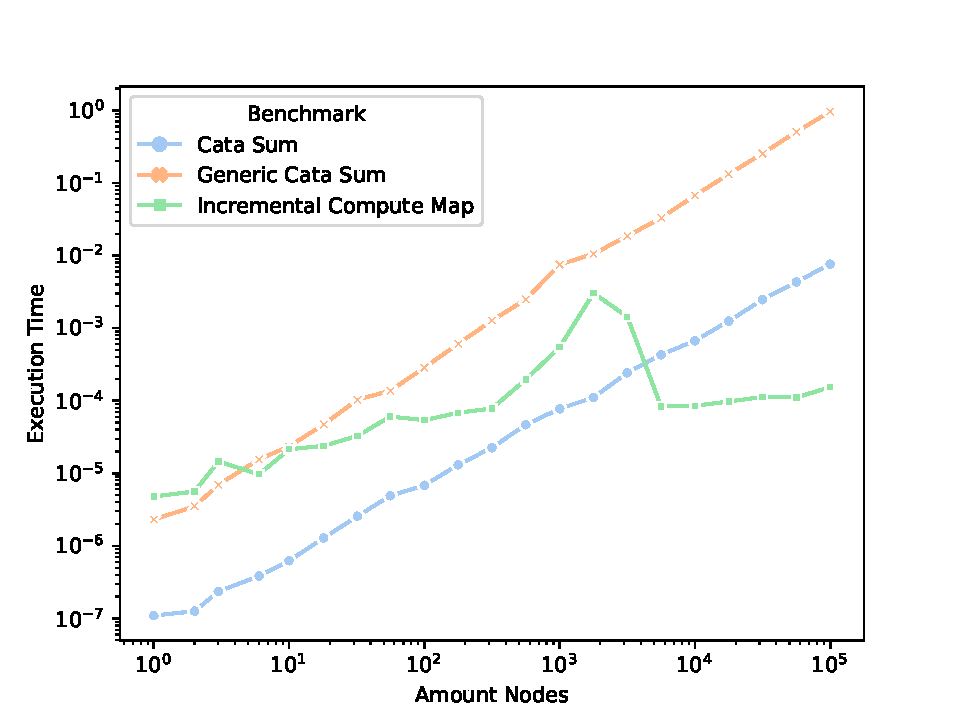
\includegraphics[width=.6\textwidth]{plots/run-2/time/all_benchmarks.pdf}
    \caption{Overview execution time}
    \label{fig-exec-time-overview}
\end{figure}

\begin{figure}[H]
    \centering
    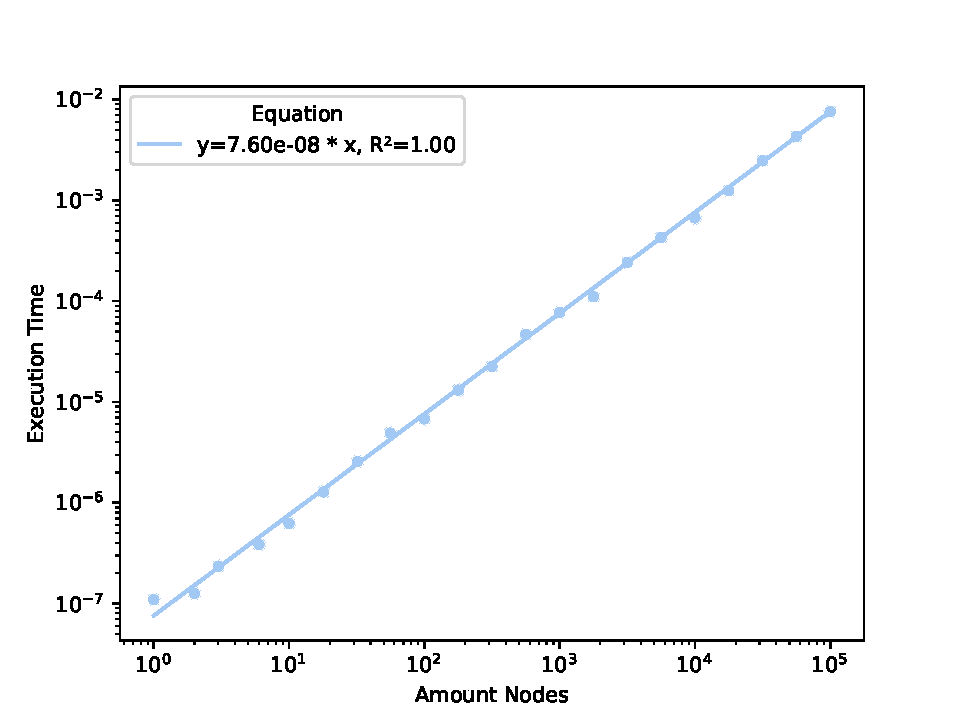
\includegraphics[width=.6\textwidth]{plots/run-2/time/benchmark_cata_sum.pdf}
    \caption{Execution time for Cata Sum}
    \label{fig-exec-time-cata-sum}
\end{figure}

\begin{figure}[H]
    \centering
    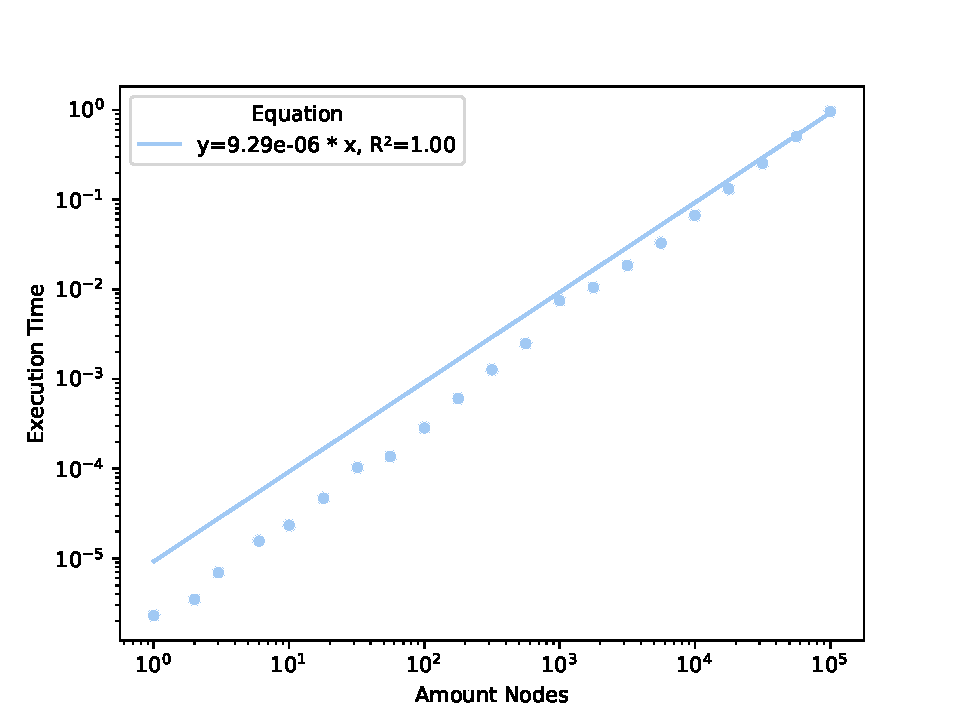
\includegraphics[width=.6\textwidth]{plots/run-2/time/benchmark_generic_cata_sum.pdf}
    \caption{Execution time for Generic Cata Sum}
    \label{fig-exec-time-gen-cata-sum}
\end{figure}

\begin{figure}[H]
    \centering
    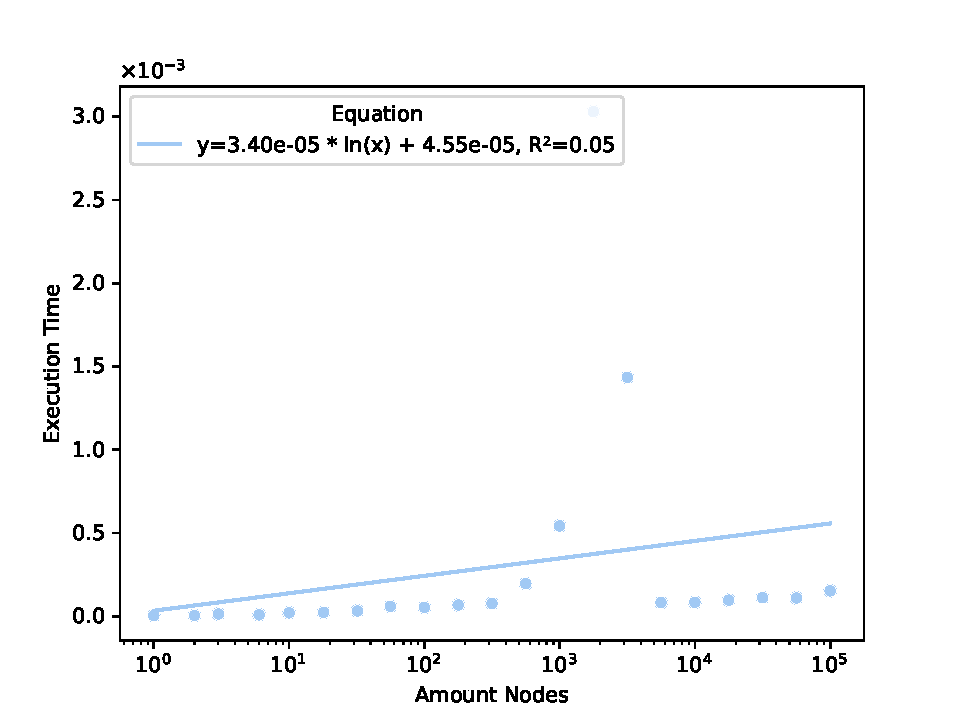
\includegraphics[width=.6\textwidth]{plots/run-2/time/benchmark_incremental_cata_sum.pdf}
    \caption{Execution time for Incremental Cata Sum}
    \label{fig-exec-time-inc-cata-sum}
\end{figure}


\subsection{Memory Usage}
\begin{figure}[H]
    \centering
    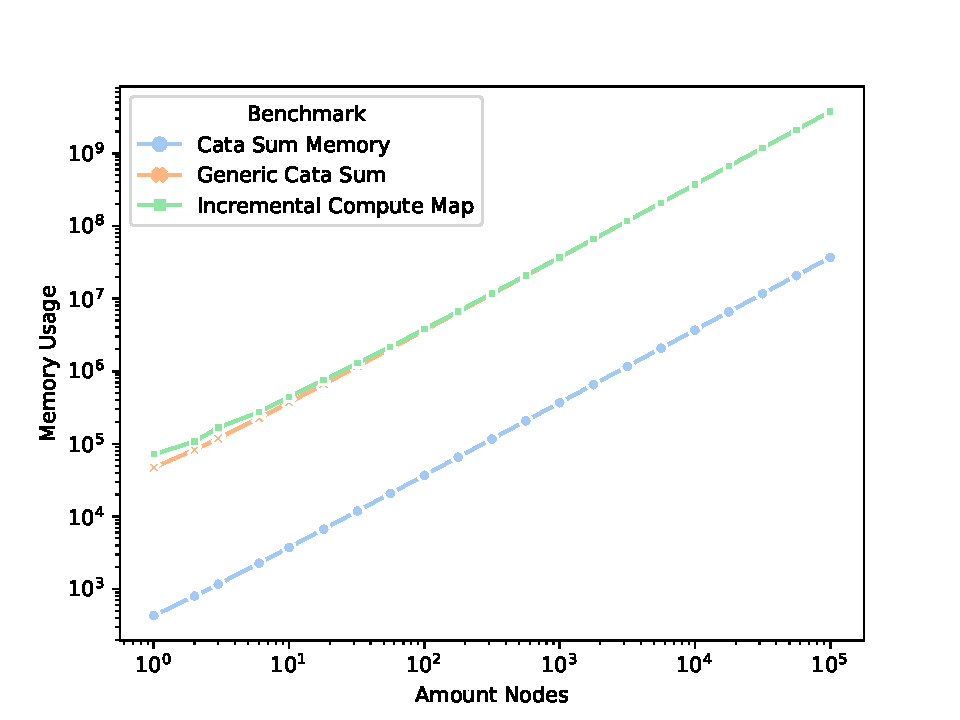
\includegraphics[width=.6\textwidth]{plots/run-2/memory/all_benchmarks.pdf}
    \caption{Overview memory usage}
    \label{fig-bytes-all-overview}
\end{figure}

\begin{figure}[H]
    \centering
    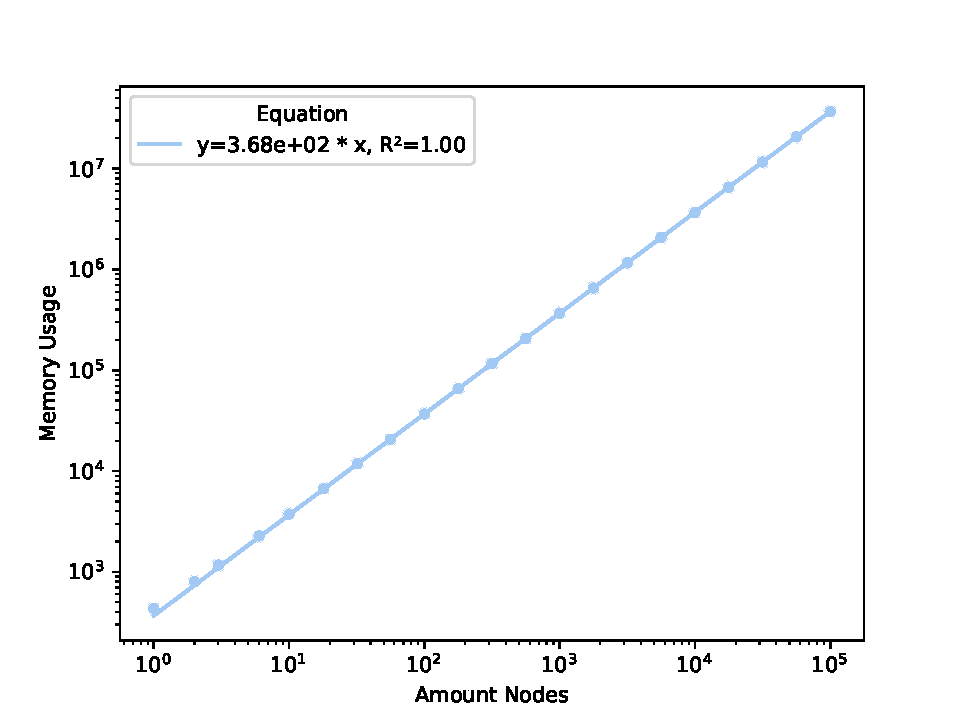
\includegraphics[width=.6\textwidth]{plots/run-2/memory/benchmark_cata_sum.pdf}
    \caption{Memory usage for Cata Sum}
    \label{fig-bytes-all-cata-sum}
\end{figure}

\begin{figure}[H]
    \centering
    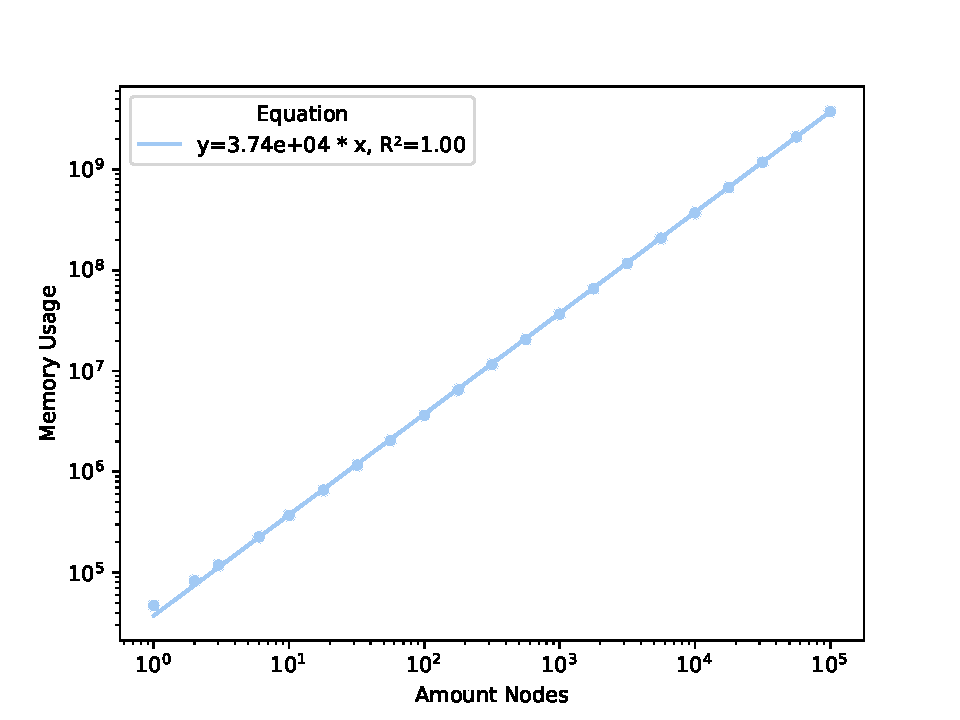
\includegraphics[width=.6\textwidth]{plots/run-2/memory/benchmark_generic_cata_sum.pdf}
    \caption{Memory usage for Generic Cata Sum}
    \label{fig-bytes-all-gen-cata-sum}
\end{figure}

\begin{figure}[H]
    \centering
    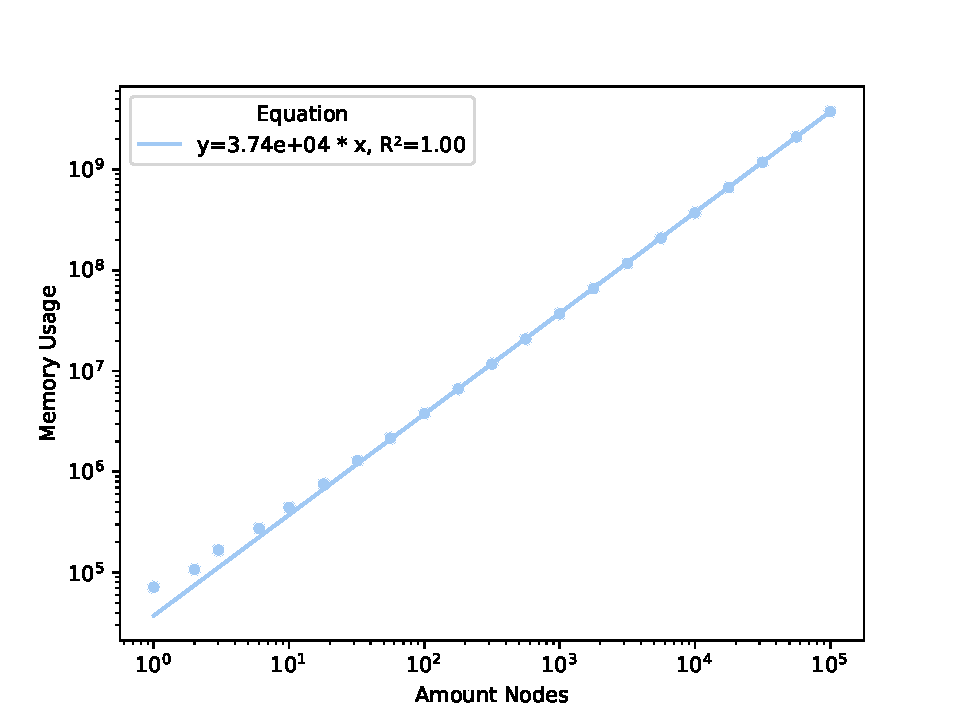
\includegraphics[width=.6\textwidth]{plots/run-2/memory/benchmark_incremental_cata_sum.pdf}
    \caption{Memory usage for Incremental Cata Sum}
    \label{fig-bytes-all-inc-cata-sum}
\end{figure}

\subsection{Comparison Memory Strategies}
\begin{figure}[H]
    \centering
    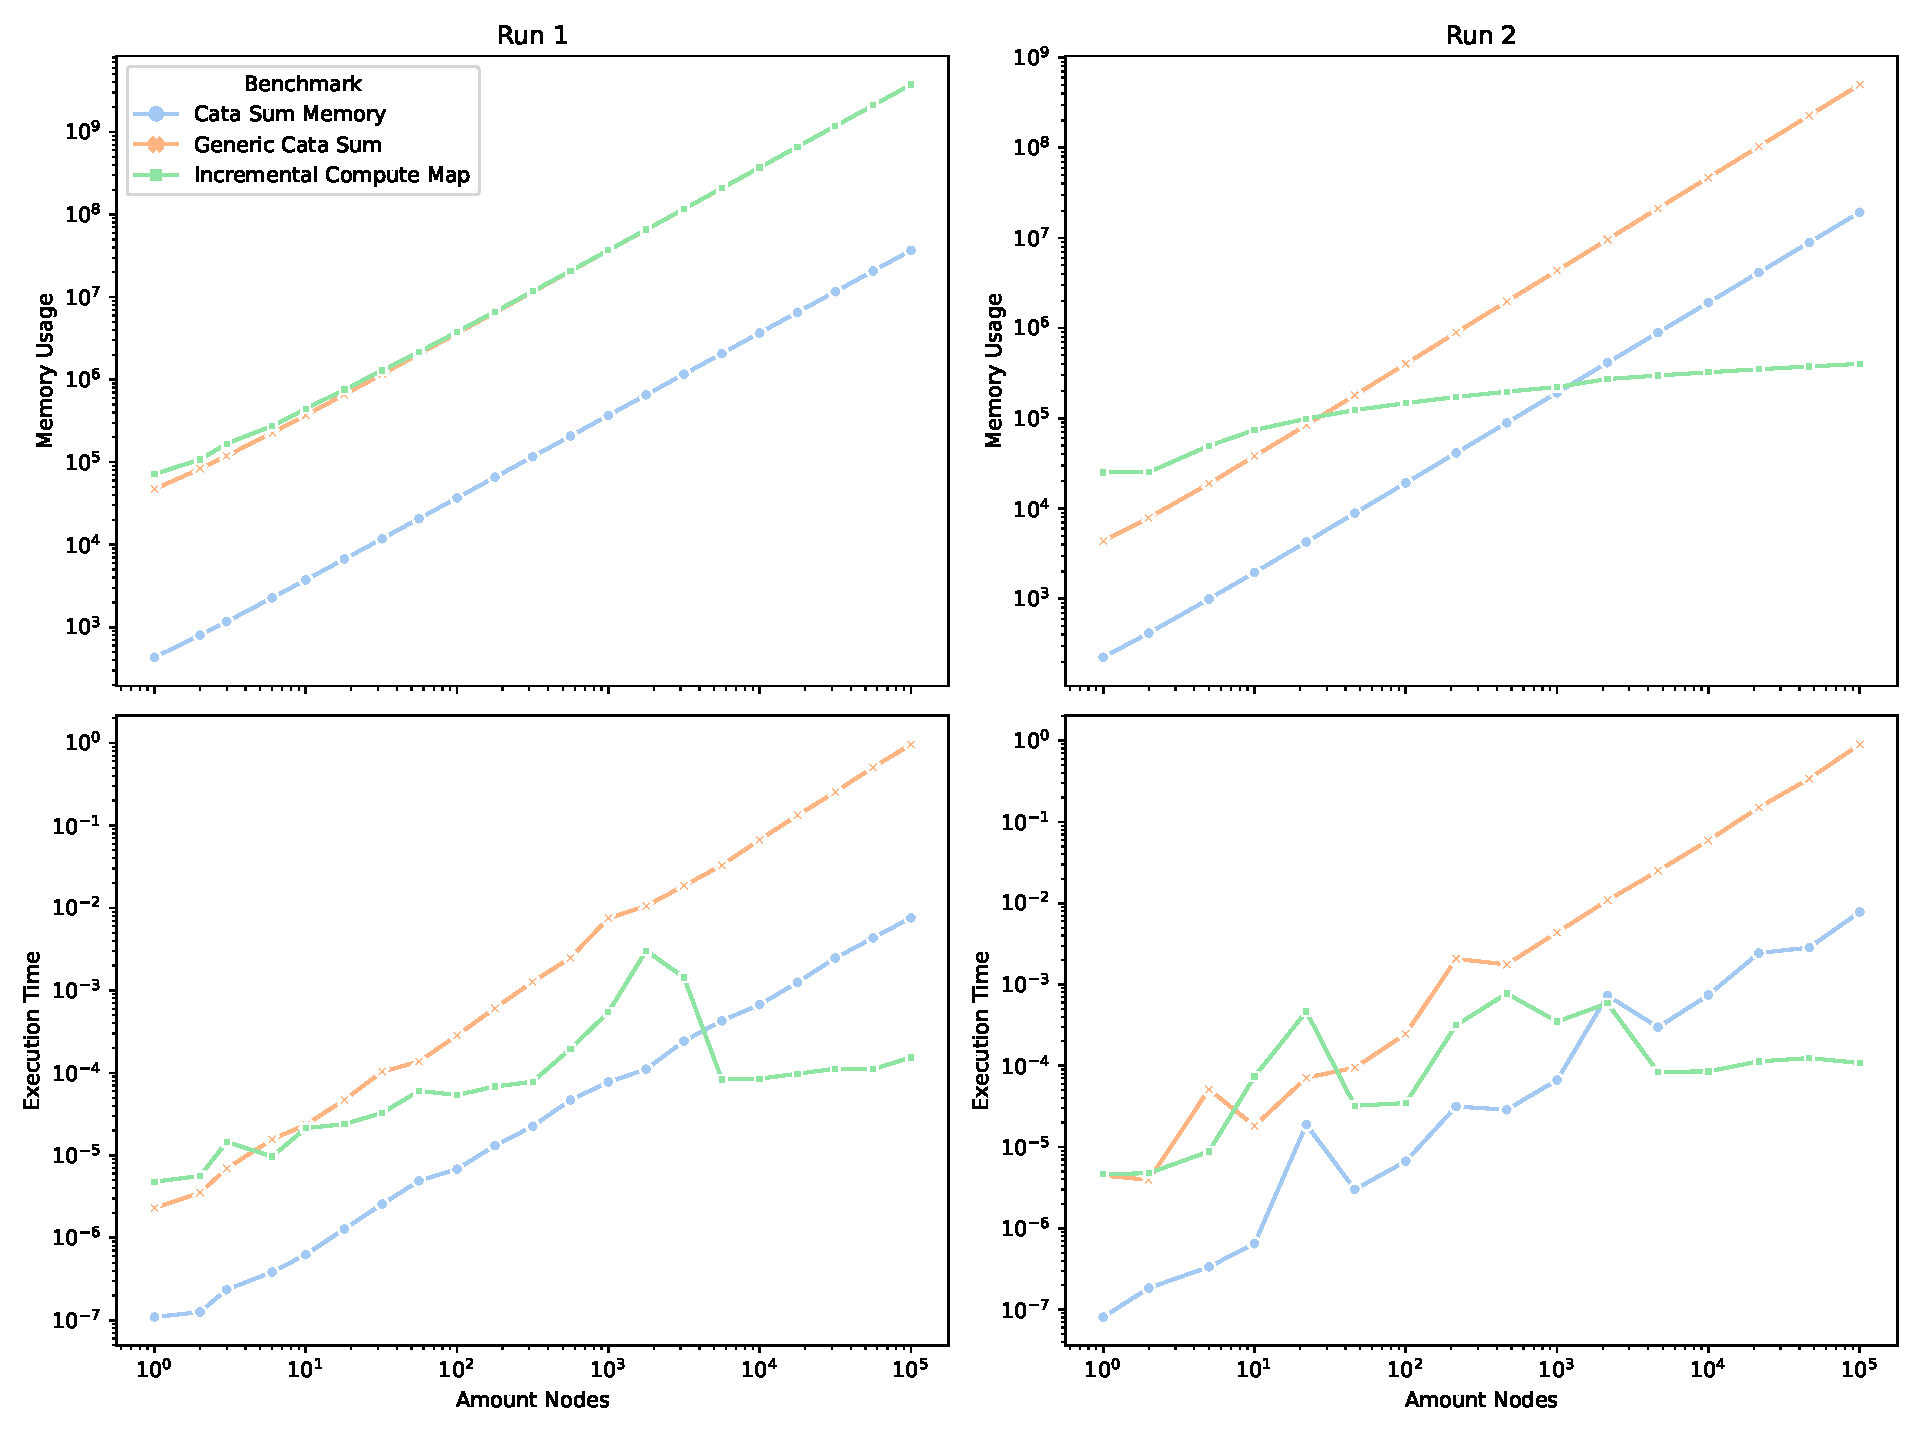
\includegraphics[width=.9\textwidth]{plots/run-2_run-1/comparison_benchmarks.pdf}
    \caption{Comparison Memory Strategy}
    \label{fig-comp-mem-strat}
\end{figure}

\newpage
\section{Conclusion}

\newpage
\section{Future Work}

% Elm, React & Victor diff algorithm

\newpage
\section{Appendix}
\appendix

\section{Implementation Memo Cata}

\subsection{Definition Generic Datatypes}
\label{app-def-generic-datatypes}
\begin{minted}{haskell}
data U r         = U
data I r         = I r                  
data K a r       = K a                  
data (:+:) f g r = L (f r) | R (g r)
data (:*:) f g r = (f r) :*: (g r) 
data C c f r     = C (f r)

newtype Fix f = In { out :: f (Fix f) }
\end{minted}

\subsection{Implementation Hashable}
\label{app-impl-hashable}
\begin{minted}{haskell}
class Hashable f where
  hash :: f (Fix (g :*: K Digest)) -> Digest

instance Hashable U where
  hash _ = digest "U"

instance (Show a) => Hashable (K a) where
  hash (K x) = digestConcat [digest "K", digest x]

instance Hashable I where
  hash (I x) = digestConcat [digest "I", getDigest x]
    where
      getDigest :: Fix (f :*: K Digest) -> Digest
      getDigest (In (_ :*: K h)) = h

instance (Hashable f, Hashable g) => Hashable (f :+: g) where
  hash (L x) = digestConcat [digest "L", hash x]
  hash (R x) = digestConcat [digest "R", hash x]

instance (Hashable f, Hashable g) => Hashable (f :*: g) where
  hash (x :*: y) = digestConcat [digest "P", hash x, hash y]

instance (Hashable f) => Hashable (C c f) where
  hash (C x) = digestConcat [digest "C", hash x]
\end{minted}

\subsection{Implementation Merkle}
\label{app-impl-merkle}
\begin{minted}{haskell}
type Merkle f = Fix (f :*: K Digest)

merkleG :: Hashable f 
        => f (Fix (g :*: K Digest)) 
        -> (f :*: K Digest) (Fix (g :*: K Digest))
merkleG f = f :*: K (hash f)

merkle :: (Regular a, Hashable (PF a), Functor (PF a)) 
       => a -> Merkle (PF a)
merkle = In . merkleG . fmap merkle . from
\end{minted}

\subsection{Implementation Cata Merkle}
\label{app-impl-cata-merkle}
\begin{minted}{haskell}
cataMerkleState :: (Functor f, Traversable f)
                => (f a -> a) -> Fix (f :*: K Digest) 
                -> State (M.Map Digest a) a
cataMerkleState alg (In (x :*: K h)) = do m <- get
  case M.lookup h m of
    Just a -> return a
    Nothing -> do y <- mapM (cataMerkleState alg) x
                  let r = alg y
                  modify (M.insert h r) >> return r

cataMerkle :: (Functor f, Traversable f)
           => (f a -> a) -> Fix (f :*: K Digest) -> (a, M.Map Digest a)
cataMerkle alg t = runState (cataMerkleState alg t) M.empty
\end{minted}

\subsection{Implementation Zipper Merkle}
\label{app-impl-zipper-merkle}
\begin{minted}{haskell}
data Loc :: * -> * where
  Loc :: (Zipper a) => Merkle a 
                    -> [Ctx (a :*: K Digest) (Merkle a)] 
                    -> Loc (Merkle a)

modify :: (a -> a) -> Loc a -> Loc a
modify f (Loc x cs) = Loc (f x) cs

updateDigest :: Hashable a => Merkle a -> Merkle a
updateDigest (In (x :*: _)) = In (merkleG x)

updateParents :: Hashable a => Loc (Merkle a) -> Loc (Merkle a)
updateParents (Loc x []) = Loc (updateDigest x) []
updateParents (Loc x cs) = updateParents
                          $ expectJust "Exception: Cannot go up"
                          $ up (Loc (updateDigest x) cs)

updateLoc :: Hashable a => (Merkle a -> Merkle a) 
                        -> Loc (Merkle a) -> Loc (Merkle a)
updateLoc f loc = if   top loc'
                  then loc'
                  else updateParents 
                       $ expectJust "Exception: Cannot go up" (up loc')
  where
    loc' = modify f loc
\end{minted}

\section{Regular}

\subsection{Zipper}
\begin{minted}{haskell}
data instance Ctx (K a) r
data instance Ctx U r
data instance Ctx (f :+: g) r = CL (Ctx f r) | CR (Ctx g r)
data instance Ctx (f :*: g) r = C1 (Ctx f r) (g r) | C2 (f r) (Ctx g r)
data instance Ctx I r = CId
data instance Ctx (C c f) r = CC (Ctx f r)
data instance Ctx (S s f) r = CS (Ctx f r)
\end{minted}

\newpage
\printbibliography

\end{document}